% --- shared colours (matplotlib tab10) ---
\definecolor{cblue}{RGB}{31,119,180}
\definecolor{cred}{RGB}{214,39,40}
\definecolor{cgreen}{RGB}{44,160,44}

% common picture options: 1 bit = 0.042 cm on both axes (square aspect)
\tikzset{bitsec/.style={x=0.042cm,y=0.042cm,font=\small}}

%======================================================================
% PANEL 1a:  Additive loss, linear attack
%======================================================================
\newcommand{\panelAddLin}{%
  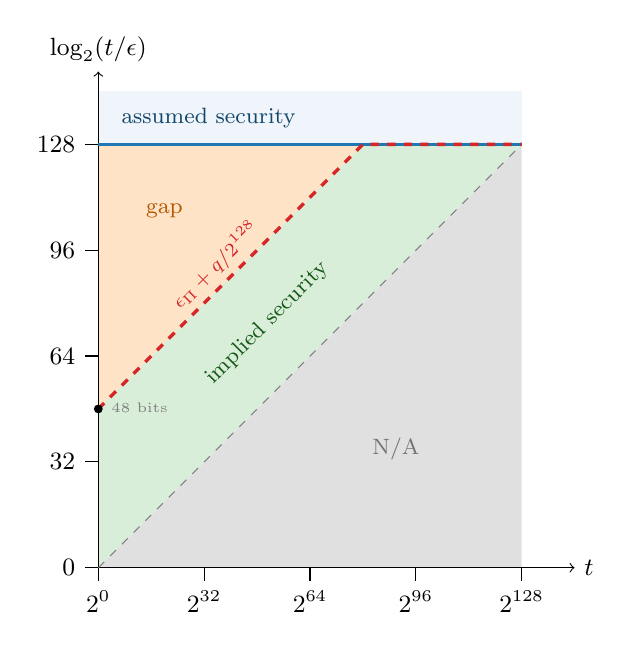
\begin{tikzpicture}[bitsec]
    \def\n{128}
    \fill[cblue!7]   (0,\n) -- (0,{\n+16}) -- (\n,{\n+16}) -- (\n,\n) -- cycle;
    \fill[black!12]  (0,0) -- (\n,\n) -- (\n,0) -- cycle;
    \fill[cgreen!18] (0,0) -- (0,48) -- (80,\n) -- (\n,\n) -- cycle;           % implied (parallel band)
    \fill[orange!22] (0,48) -- (0,\n) -- (80,\n) -- cycle;                     % gap
    \draw[->] (0,0) -- (0,{\n+22}) node[above] {$\log_2(t/\epsilon)$};
    \draw[->] (0,0) -- ({\n+16},0) node[right] {$t$};
    \foreach \x in {0,32,64,96,128} \draw (\x,0)--(\x,-4) node[below] {$2^{\x}$};
    \foreach \y in {0,32,64,96,128} \draw (0,\y)--(-4,\y) node[left] {$\y$};
    \draw[gray,dashed] (0,0) -- (\n,\n);
    \draw[cblue,very thick] (0,\n) -- (\n,\n);
    \draw[cred,very thick,dashed] (0,48) -- (80,\n) -- (\n,\n);
    \fill (0,48) circle (1.6pt);
    \node[anchor=south west,font=\tiny,gray] at (1,44) {$48$ bits};
    \node[cblue!60!black,anchor=west,font=\footnotesize] at (4,{\n+8}) {assumed security};
    \node[cred,rotate=45,anchor=south,font=\scriptsize] at (40,87) {$\epsilon_\Pi+q/2^{128}$};
    \node[orange!70!black,font=\footnotesize] at (20,108) {gap};
    \node[cgreen!55!black,rotate=45,font=\footnotesize] at (51,74) {implied security};
    \node[black!55,align=center,font=\footnotesize] at (90,36) {N/A};
  \end{tikzpicture}
}

%======================================================================
% PANEL 1b:  Additive loss, quadratic attack
%======================================================================
\newcommand{\panelAddQuad}{%
  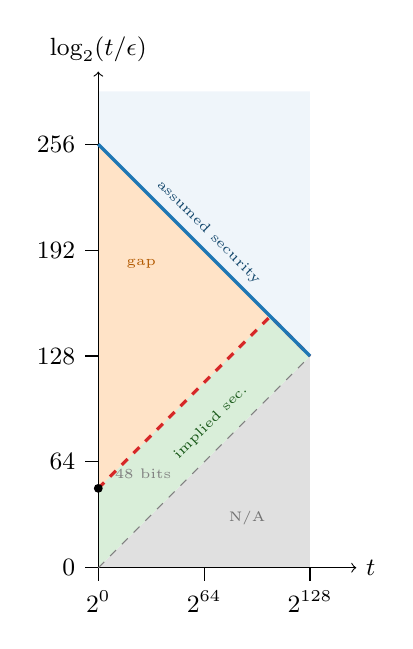
\begin{tikzpicture}[bitsec]
    \def\n{128}\def\m{64}
    \fill[cblue!7]   (0,\n) -- (0,{\n+16}) -- (\m,{\n+16}) -- (\m,\m) -- cycle;
    \fill[black!12]  (0,0) -- (\m,\m) -- (\m,0) -- cycle;
    \fill[cgreen!18] (0,0) -- (0,24) -- (52,76) -- (\m,\m) -- cycle;
    \fill[orange!22] (0,24) -- (0,\n) -- (52,76) -- cycle;
    \draw[->] (0,0) -- (0,{\n+22}) node[above] {$\log_2(t/\epsilon)$};
    \draw[->] (0,0) -- ({\m+14},0) node[right] {$t$};
    \foreach \x in {0,64,128} \draw ({\x/2},0)--({\x/2},-4) node[below] {$2^{\x}$};
    \foreach \y in {0,64,128,192,256} \draw (0,{\y/2})--(-4,{\y/2}) node[left] {$\y$};
    \draw[gray,dashed] (0,0) -- (\m,\m);
    \draw[cred,very thick,dashed] (0,24) -- (52,76) -- (\m,\m);
    \draw[cblue,very thick] (0,\n) -- (\m,\m);
    \fill (0,24) circle (1.6pt);
    \node[anchor=south west,font=\tiny,gray] at (1,24) {$\,48$ bits};
    \node[cblue!60!black,rotate=-45,anchor=south,font=\tiny] at (30,98) {assumed security};
    \node[orange!70!black,font=\tiny] at (13,92) {gap};
    \node[cgreen!55!black,rotate=45,font=\tiny] at (34,44) {implied sec.};
    \node[black!55,font=\tiny] at (45,15) {N/A};
  \end{tikzpicture}
}

%======================================================================
% PANEL 1c:  Additive loss, cubic attack
%======================================================================
\newcommand{\panelAddCube}{%
  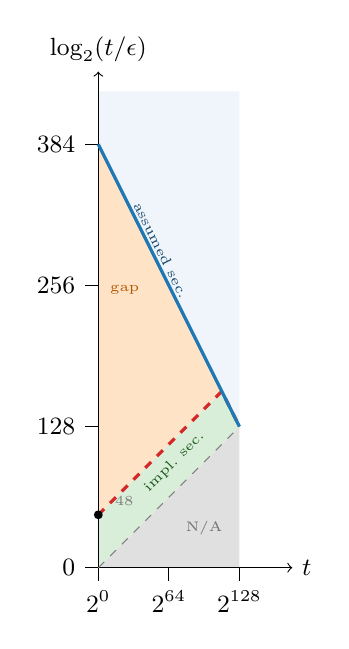
\begin{tikzpicture}[bitsec]
    \def\n{128}
    \fill[cblue!7]   (0,\n) -- (0,{\n+16}) -- ({\n/3},{\n+16}) -- ({\n/3},{\n/3}) -- cycle;
    \fill[black!12]  (0,0) -- ({\n/3},{\n/3}) -- ({\n/3},0) -- cycle;
    \fill[cgreen!18] (0,0) -- (0,16) -- (37.333,53.333) -- ({\n/3},{\n/3}) -- cycle;
    \fill[orange!22] (0,16) -- (0,\n) -- (37.333,53.333) -- cycle;
    \draw[->] (0,0) -- (0,{\n+22}) node[above] {$\log_2(t/\epsilon)$};
    \draw[->] (0,0) -- ({\n/3+16},0) node[right] {$t$};
    \foreach \x in {0,64,128} \draw ({\x/3},0)--({\x/3},-4) node[below] {$2^{\x}$};
    \foreach \y in {0,128,256,384} \draw (0,{\y/3})--(-4,{\y/3}) node[left] {$\y$};
    \draw[gray,dashed] (0,0) -- ({\n/3},{\n/3});
    \draw[cred,very thick,dashed] (0,16) -- (37.333,53.333) -- ({\n/3},{\n/3});
    \draw[cblue,very thick] (0,\n) -- ({\n/3},{\n/3});
    \fill (0,16) circle (1.6pt);
    \node[anchor=south west,font=\tiny,gray] at (1,16) {$\,48$};
    \node[cblue!60!black,rotate=-63.43,anchor=south,font=\tiny] at (15,94) {assumed sec.};
    \node[orange!70!black,font=\tiny] at (8,84) {gap};
    \node[cgreen!55!black,rotate=45,font=\tiny] at (23,32) {impl.\ sec.};
    \node[black!55,font=\tiny] at (32,12) {N/A};
  \end{tikzpicture}
}

%======================================================================
% PANEL 2a:  Multiplicative loss, linear attack
%======================================================================
\newcommand{\panelMultLin}{%
  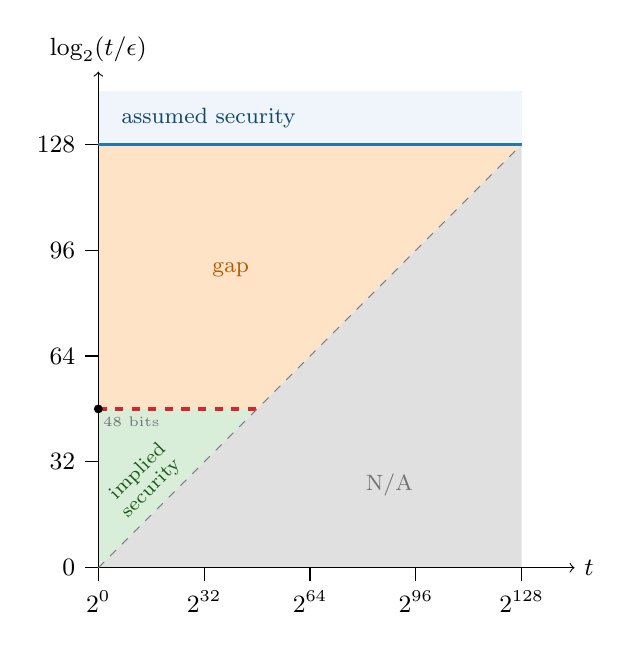
\begin{tikzpicture}[bitsec]
    \def\n{128}\def\l{80}
    \fill[cblue!7]   (0,\n) -- (0,{\n+16}) -- (\n,{\n+16}) -- (\n,\n) -- cycle;
    \fill[orange!22] (0,{\n-\l}) -- ({\n-\l},{\n-\l}) -- (\n,\n) -- (0,\n) -- cycle;
    \fill[cgreen!18] (0,0) -- (0,{\n-\l}) -- ({\n-\l},{\n-\l}) -- cycle;
    \fill[black!12]  (0,0) -- (\n,\n) -- (\n,0) -- cycle;
    \draw[->] (0,0) -- (0,{\n+22}) node[above] {$\log_2(t/\epsilon)$};
    \draw[->] (0,0) -- ({\n+16},0) node[right] {$t$};
    \foreach \x in {0,32,64,96,128} \draw (\x,0)--(\x,-4) node[below] {$2^{\x}$};
    \foreach \y in {0,32,64,96,128} \draw (0,\y)--(-4,\y) node[left] {$\y$};
    \draw[cblue,very thick] (0,\n) -- (\n,\n);
    \draw[cred,very thick,dashed] (0,{\n-\l}) -- ({\n-\l},{\n-\l});
    \draw[gray,dashed] (0,0) -- (\n,\n);
    \fill (0,{\n-\l}) circle (1.6pt);
    \node[black!55,font=\tiny] at (10,44) {$48$ bits};
    %\node[gray,rotate=45,anchor=south,font=\footnotesize] at (104,104) {$\epsilon=1$};
    %\node[cred,rotate=26.57,anchor=south,font=\footnotesize] at (58,90) {$\kappa_A=\tfrac12(\tau+n)$};
    %\node[cblue,anchor=south,font=\footnotesize] at (96,129) {$\kappa_B=n$};
    \node[cblue!60!black,anchor=west,font=\footnotesize] at (4,{\n+8}) {assumed security};
    \node[orange!70!black,font=\footnotesize] at (40,90) {gap};
    %\node[cgreen!55!black,font=\footnotesize] at (17,37) {implied};
    \node[cgreen!55!black,rotate=45,font=\scriptsize] at (12,29) {implied};
    \node[cgreen!55!black,rotate=45,font=\scriptsize] at (16,24) {security};
    \node[black!55,align=center,font=\footnotesize] at (88,25) {N/A};
  \end{tikzpicture}
}

%======================================================================
% PANEL 2b:  Multiplicative loss, quadratic attack
%======================================================================
\newcommand{\panelMultQuad}{%
  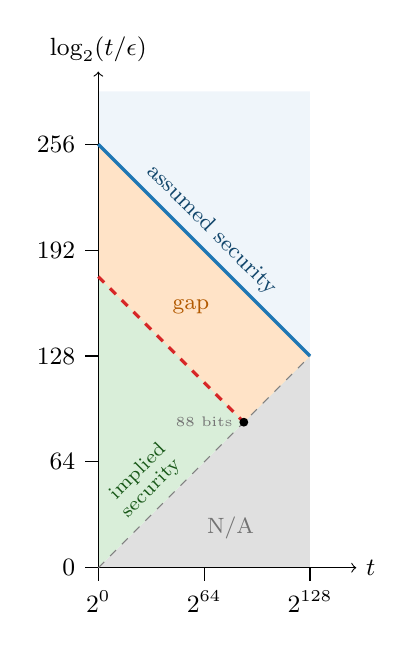
\begin{tikzpicture}[bitsec]
    \def\n{128}\def\m{64}\def\l{40}
    \fill[cblue!7]   (0,\n) -- (0,{\n+16}) -- (\m,{\n+16}) -- (\m,\m) -- cycle;
    \fill[black!12]  (0,0) -- (\m,\m) -- (\m,0) -- cycle;
    \fill[cgreen!18] (0,0) -- (0,{\n-\l}) -- (\m,\m) -- cycle;
    \fill[orange!22] (0,{\n-\l}) -- (0,\n) -- (\m,\m) -- ({(\n-\l)/2},{(\n-\l)/2}) -- cycle;
    \draw[->] (0,0) -- (0,{\n+22}) node[above] {$\log_2(t/\epsilon)$};
    \draw[->] (0,0) -- ({\m+14},0) node[right] {$t$};
    \foreach \x in {0,64,128} \draw ({\x/2},0)--({\x/2},-4) node[below] {$2^{\x}$};
    \foreach \y in {0,64,128,192,256} \draw (0,{\y/2})--(-4,{\y/2}) node[left] {$\y$};
    \draw[cblue,very thick] (0,\n) -- (\m,\m);
    \draw[cred,very thick,dashed] (0,{\n-\l}) -- ({(\n-\l)/2},{(\n-\l)/2});
    \draw[gray,dashed] (0,0) -- (\m,\m);
    \fill ({(\n-\l)/2},{(\n-\l)/2}) circle (1.6pt);
    %\node[cblue,rotate=-45,anchor=south,font=\footnotesize] at (24,104) {$\kappa_B=n-\tau$};
    %\node[cred,anchor=south,font=\footnotesize] at (18,65) {$\kappa_A=n/2$};
    %\node[gray,rotate=45,anchor=south,font=\footnotesize] at (28,28) {$\epsilon=1$};
    \node[cblue!60!black,rotate=-45,anchor=south,font=\footnotesize] at (30,98) {assumed security};
    \node[orange!70!black,font=\footnotesize] at (28,79) {gap};
    %\node[cgreen!55!black,font=\footnotesize] at (18,44) {implied};
    \node[black!55,font=\tiny] at (32,44) {$88$ bits};
    \node[cgreen!55!black,rotate=45,font=\scriptsize] at (12,29) {implied};
    \node[cgreen!55!black,rotate=45,font=\scriptsize] at (16,24) {security};
    \node[black!55,font=\footnotesize] at (40,12) {N/A};
  \end{tikzpicture}
}

%======================================================================
% PANEL 2c:  Multiplicative loss, cubic attack
%======================================================================
\newcommand{\panelMultCube}{%
  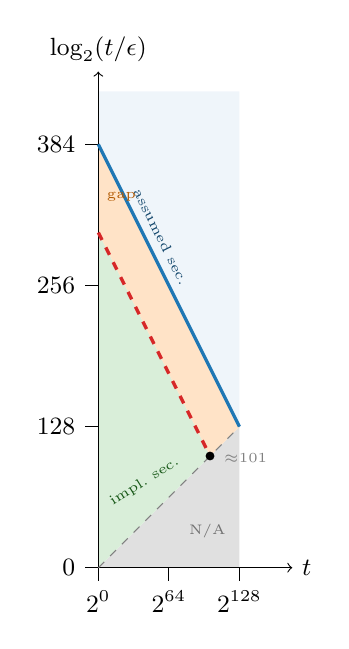
\begin{tikzpicture}[bitsec]
    \def\n{128}
    \fill[cblue!7]   (0,\n) -- (0,{\n+16}) -- ({\n/3},{\n+16}) -- ({\n/3},{\n/3}) -- cycle;
    \fill[black!12]  (0,0) -- ({\n/3},{\n/3}) -- ({\n/3},0) -- cycle;
    \fill[cgreen!18] (0,0) -- (0,101.333) -- (33.778,33.778) -- cycle;
    \fill[orange!22] (0,101.333) -- (33.778,33.778) -- ({\n/3},{\n/3}) -- (0,\n) -- cycle;
    \draw[->] (0,0) -- (0,{\n+22}) node[above] {$\log_2(t/\epsilon)$};
    \draw[->] (0,0) -- ({\n/3+16},0) node[right] {$t$};
    \foreach \x in {0,64,128} \draw ({\x/3},0)--({\x/3},-4) node[below] {$2^{\x}$};
    \foreach \y in {0,128,256,384} \draw (0,{\y/3})--(-4,{\y/3}) node[left] {$\y$};
    \draw[gray,dashed] (0,0) -- ({\n/3},{\n/3});
    \draw[cred,very thick,dashed] (0,101.333) -- (33.778,33.778);
    \draw[cblue,very thick] (0,\n) -- ({\n/3},{\n/3});
    \fill (33.778,33.778) circle (1.6pt);
    \node[anchor=west,font=\tiny,gray] at (35,33) {$\approx$101};
    \node[cblue!60!black,rotate=-63.43,anchor=south,font=\tiny] at (15,98) {assumed sec.};
    \node[orange!70!black,font=\tiny] at (7,112) {gap};
    \node[cgreen!55!black,rotate=32,font=\tiny] at (14,26) {impl.\ sec.};
    \node[black!55,font=\tiny] at (33,11) {N/A};
  \end{tikzpicture}
}

%======================================================================
% PANEL 3a:  Square-root loss, linear attack
%======================================================================
\newcommand{\panelRootLin}{%
  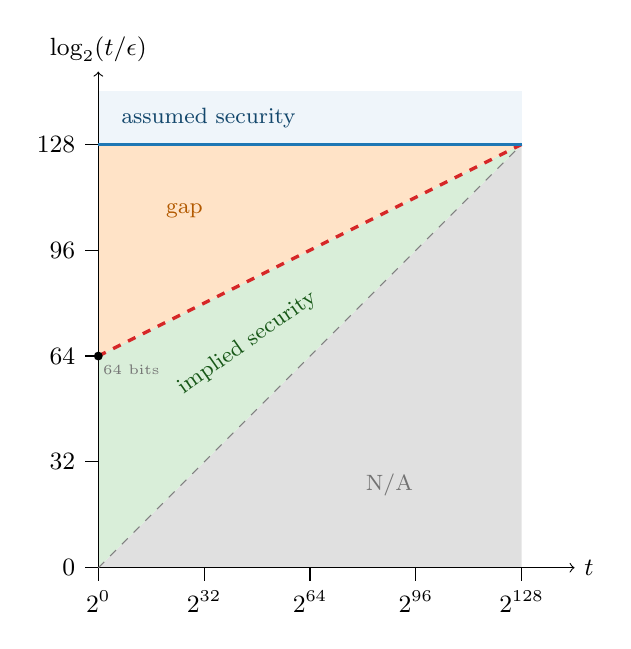
\begin{tikzpicture}[bitsec]
    \def\n{128}
    \fill[cblue!7]   (0,\n) -- (0,{\n+16}) -- (\n,{\n+16}) -- (\n,\n) -- cycle;
    \fill[black!12]  (0,0) -- (\n,\n) -- (\n,0) -- cycle;
    \fill[cgreen!18] (0,0) -- (0,{\n/2}) -- (\n,\n) -- cycle;
    \fill[orange!22] (0,{\n/2}) -- (0,\n) -- (\n,\n) -- cycle;
    \draw[->] (0,0) -- (0,{\n+22}) node[above] {$\log_2(t/\epsilon)$};
    \draw[->] (0,0) -- ({\n+16},0) node[right] {$t$};
    \foreach \x in {0,32,64,96,128} \draw (\x,0)--(\x,-4) node[below] {$2^{\x}$};
    \foreach \y in {0,32,64,96,128} \draw (0,\y)--(-4,\y) node[left] {$\y$};
    \draw[gray,dashed] (0,0) -- (\n,\n);
    \draw[cred,very thick,dashed] (0,{\n/2}) -- (\n,\n);
    \draw[cblue,very thick] (0,\n) -- (\n,\n);
    \fill (0,64) circle (1.6pt);
    \node[black!55,font=\tiny] at (10,60) {$64$ bits};
    %\node[gray,rotate=45,anchor=south,font=\footnotesize] at (104,104) {$\epsilon=1$};
    %\node[cred,rotate=26.57,anchor=south,font=\footnotesize] at (58,90) {$\kappa_A=\tfrac12(\tau+n)$};
    %\node[cblue,anchor=south,font=\footnotesize] at (96,129) {$\kappa_B=n$};
    \node[cblue!60!black,anchor=west,font=\footnotesize] at (4,{\n+8}) {assumed security};
    \node[orange!70!black,font=\footnotesize] at (26,108) {gap};
    \node[cgreen!55!black,rotate=35,font=\footnotesize] at (45,68) {implied security};
    \node[black!55,align=center,font=\footnotesize] at (88,25) {N/A};
  \end{tikzpicture}
}

%======================================================================
% PANEL 3b:  Square-root loss, quadratic attack
%======================================================================
\newcommand{\panelRootQuad}{%
  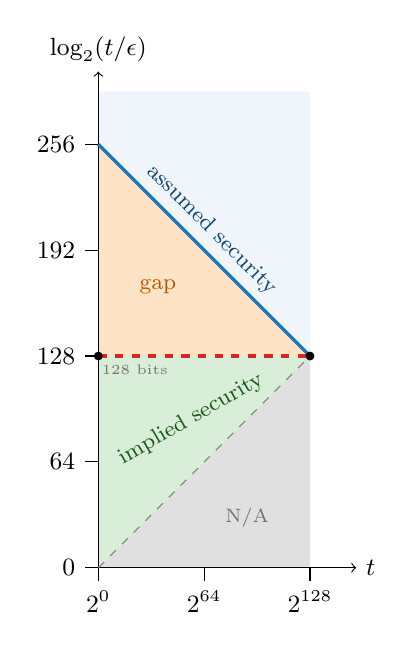
\begin{tikzpicture}[bitsec]
    \def\n{128}\def\m{64}
    \fill[cblue!7]   (0,\n) -- (0,{\n+16}) -- (\m,{\n+16}) -- (\m,\m) -- cycle;
    \fill[black!12]  (0,0) -- (\m,\m) -- (\m,0) -- cycle;
    \fill[cgreen!18] (0,0) -- (0,\m) -- (\m,\m) -- cycle;
    \fill[orange!22] (0,\m) -- (0,\n) -- (\m,\m) -- cycle;
    \draw[->] (0,0) -- (0,{\n+22}) node[above] {$\log_2(t/\epsilon)$};
    \draw[->] (0,0) -- ({\m+14},0) node[right] {$t$};
    \foreach \x in {0,64,128} \draw ({\x/2},0)--({\x/2},-4) node[below] {$2^{\x}$};
    \foreach \y in {0,64,128,192,256} \draw (0,{\y/2})--(-4,{\y/2}) node[left] {$\y$};
    \draw[gray,dashed] (0,0) -- (\m,\m);
    \draw[cblue,very thick] (0,\n) -- (\m,\m);
    \draw[cred,very thick,dashed] (0,\m) -- (\m,\m);
    \fill (0,\m) circle (1.6pt);
    \fill (\m,\m) circle (1.6pt);
    \node[black!55,font=\tiny] at (11,60) {$128$ bits};
    %\node[cblue,rotate=-45,anchor=south,font=\footnotesize] at (24,104) {$\kappa_B=n-\tau$};
    %\node[cred,anchor=south,font=\footnotesize] at (18,65) {$\kappa_A=n/2$};
    %\node[gray,rotate=45,anchor=south,font=\footnotesize] at (28,28) {$\epsilon=1$};
    \node[cblue!60!black,rotate=-45,anchor=south,font=\footnotesize] at (30,98) {assumed security};
    \node[orange!70!black,font=\footnotesize] at (18,85) {gap};
    \node[cgreen!55!black,rotate=30,font=\footnotesize] at (28,45) {implied security};
    \node[black!55,font=\scriptsize] at (45,15) {N/A};
  \end{tikzpicture}
}

%======================================================================
% PANEL 3c:  Square-root loss, qubic attack
%======================================================================
\newcommand{\panelRootCube}{%
  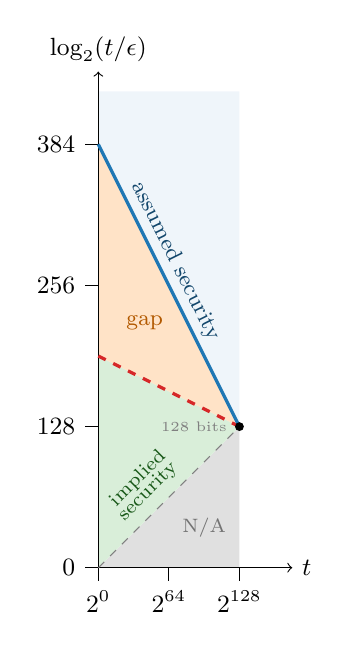
\begin{tikzpicture}[bitsec]
    \def\n{128}
    \fill[cblue!7]   (0,\n) -- (0,{\n+16}) -- ({\n/3},{\n+16}) -- ({\n/3},{\n/3}) -- cycle;
    \fill[black!12]  (0,0) -- ({\n/3},{\n/3}) -- ({\n/3},0) -- cycle;
    \fill[cgreen!18] (0,0) -- (0,{\n/2}) -- ({\n/3},{\n/3}) -- cycle;
    \fill[orange!22] (0,{\n/2}) -- (0,\n) -- ({\n/3},{\n/3}) -- cycle;
    \draw[->] (0,0) -- (0,{\n+22}) node[above] {$\log_2(t/\epsilon)$};
    \draw[->] (0,0) -- ({\n/3+16},0) node[right] {$t$};
    \foreach \x in {0,64,128} \draw ({\x/3},0)--({\x/3},-4) node[below] {$2^{\x}$};
    \foreach \y in {0,128,256,384} \draw (0,{\y/3})--(-4,{\y/3}) node[left] {$\y$};
    \draw[gray,dashed] (0,0) -- ({\n/3},{\n/3});
    \draw[cred,very thick,dashed] (0,{\n/2}) -- ({\n/3},{\n/3});
    \draw[cblue,very thick] (0,\n) -- ({\n/3},{\n/3});
    \fill ({\n/3},{\n/3}) circle (1.6pt);
    \node[anchor=west,font=\tiny,gray] at (16,{\n/3}) {128 bits};
    \node[cblue!60!black,rotate=-63.43,anchor=south,font=\footnotesize] at (18,90) {assumed security};
    \node[orange!70!black,font=\footnotesize] at (14,74) {gap};
    \node[cgreen!55!black,rotate=45,font=\scriptsize] at (12,27) {implied};
    \node[cgreen!55!black,rotate=45,font=\scriptsize] at (15,23) {security};
    \node[black!55,font=\scriptsize] at (32,12) {N/A};
  \end{tikzpicture}
}

%
\resizebox{\textwidth}{!}{
  \begin{tabular}{@{}c@{\hspace{1em}}c@{\hspace{1em}}c@{}}
    \panelcap{\panelAddLin}{
      (a) Additive loss, linear attack
    }
    & \panelcap{\panelAddQuad}{
      (b) (WIP) Additive loss, quadratic attack
    } 
    & \panelcap{\panelAddCube}{
      (c) (WIP) Additive loss, cubic attack
    } \\[30pt]
    \panelcap{\panelMultLin}{
      (d) Multiplicative loss, linear attack
    }
    & \panelcap{\panelMultQuad}{
      (e) Multiplicative loss, quadratic attack
    }
    & \panelcap{\panelMultCube}{
      (f) (WIP) Multiplicative loss, cubic attack
    } \\[30pt]
    \panelcap{\panelRootLin}{
      (g) Square-root loss, linear attack
    }
    & \panelcap{\panelRootQuad}{
      (h) Square-root loss, quadratic attack
    }
    & \panelcap{\panelRootCube}{
      (i) Square-root loss, cubic attack
    } \\[30pt]
  \end{tabular}
}
